\documentclass{beamer}

\usepackage[utf8]{inputenc}
\usepackage[T1]{fontenc}
\usepackage{times}
\usepackage{graphicx}

%\usetheme[hideothersubsections, width = 28mm]{Berkeley}
%\usecolortheme{seahorse}
%\usecolortheme{lily}
\setbeamertemplate{navigation symbols}

\title{Optimal Fitting of Planar Curves to Prescribed Constraints}
\author{Julian Asamer, Julian Brunner}
\date{\today}

\begin{document}

	\begin{frame}
		\titlepage
	\end{frame}

	\section{Introduction}

		\begin{frame}
			\frametitle{Introduction}
			\begin{itemize}
				\item vector grapics are widely used
				\item 2D vector graphics primitives are curves
				\item design process of curves is very important
				\item designing curves with current tools can be frustrating
				% artist has a hard time to make the curve look the way he wants to
				% often unclear why
				% it's hard to communicate intentions
				\item research has been done in different direction with little impact
				\item our objective: improved curve design process
				% identify nature and cause of shortcomings in current curve design tools 
				% develop a better curve design tool
			\end{itemize}
		\end{frame}
		
	\section{Problem Analysis}
	
		\begin{frame}
			\frametitle{The Curve Design Process}
			\begin{itemize}
				\item obtain source curve
				% as real or mental image, obviously software-independent
				\item extract properties from the source curve 
				\item provide them to the software
				% strongly dependent on curve design tool - the software dictates which properties can be entered
				\item the software derives a curve
				% if the curve is not precisely specified, a fairment measure is used to derive the most likely result curve
				% iteration over steps 2-4 to adjust the curve until satisfactory alignment with the source curve is reached
			\end{itemize}
		\end{frame}
		
		\begin{frame}
			\frametitle{Usability Criteria for Curve Design Tools}
			\begin{itemize}
				% curve design tools can affect the design process by choosing specification language and fairness measure, and practical ability to derive curves from them
				\item specification language + fairness measure = description language
				\item specification language should be
				\begin{itemize}
					\item expressive
					% easy to handle for humans
					\item easy
					% allow efficient communication of intent
					\item efficient
				\end{itemize}
				\item fairness measure should ensure
				\begin{itemize}
					% capture intuitive notions of smoothness
					\item smoothness
					% select curves that are minimal in respect to the specification
					\item select minimal curves
				\end{itemize}
			\end{itemize}
		\end{frame}
		
		\begin{frame}
			\frametitle{Criteria for Assessing the Usability of a Curve Design Tool}
			\begin{enumerate}
				% expressiveness of the specification language
				\item expressiveness
				% human ability to `read' the specification language from curves
				\item simplicity of finding specifications of curves
				% human ability to `speak' the specification language to the software
				\item simplicity of communicating intent
				% smoothness of curves selected by the fairness measure
				\item smoothness
				% minimality of curves selected by the fairness measure
				\item minimality
				% software's ability to derive curves from descriptions
				\item ability to derive curves from descriptions
			\end{enumerate}
		\end{frame}
		
	\section{Existing Curve Design Tools}
		\begin{frame}
			\frametitle{Bézier Splines}
			\begin{itemize}
				\item most commonly used
				\item edited by directly modifying coefficient points
				% the user can effectively specify start and end points as well as start and end velocities (which are proportional to the distance between the second and the first as well as the fourth and third point)
				% user supplies start and end point and velocity; fairness measure always chooses cubic Bézier spline.
				% which is uniquely specified
				\item most criteria fulfilled nicely except
				\item the fairness measure's smoothness 
				\begin{itemize}
					\item curvature continuity is not guaranteed across segments
					\item it is very hard to choose coefficient points in a way that results in curvature continuity.
				\end{itemize}
				\item the expressiveness of the specification language
				\begin{itemize}
					\item curvature cannot be specified directly
					\item constant/linearly changing curvature cannot be specified
					\item circular arcs/spirals are very hard to specify
				\end{itemize}
			\end{itemize}
		\end{frame}
		
		\begin{frame}
			\frametitle{Introduction}
			\begin{itemize}
				\item Foo
			\end{itemize}
			\begin{centering}
				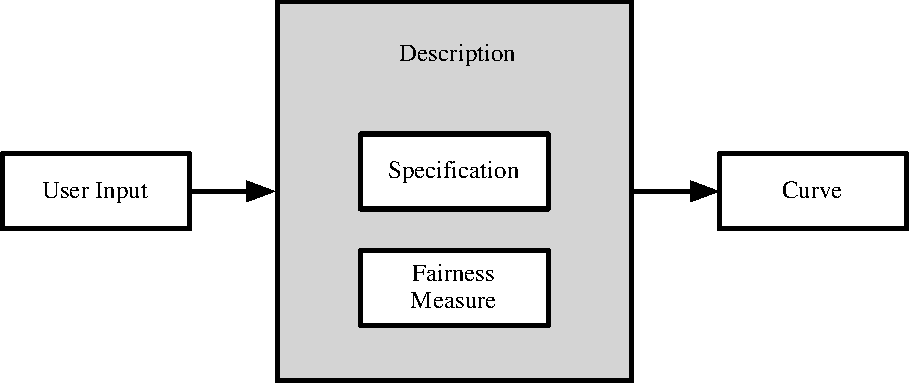
\includegraphics[width=\textwidth]{../resources/description-based_curves.pdf}\\
			\end{centering}
		\end{frame}

\end{document}
